\begin{figure}[htbp]
  \centering
  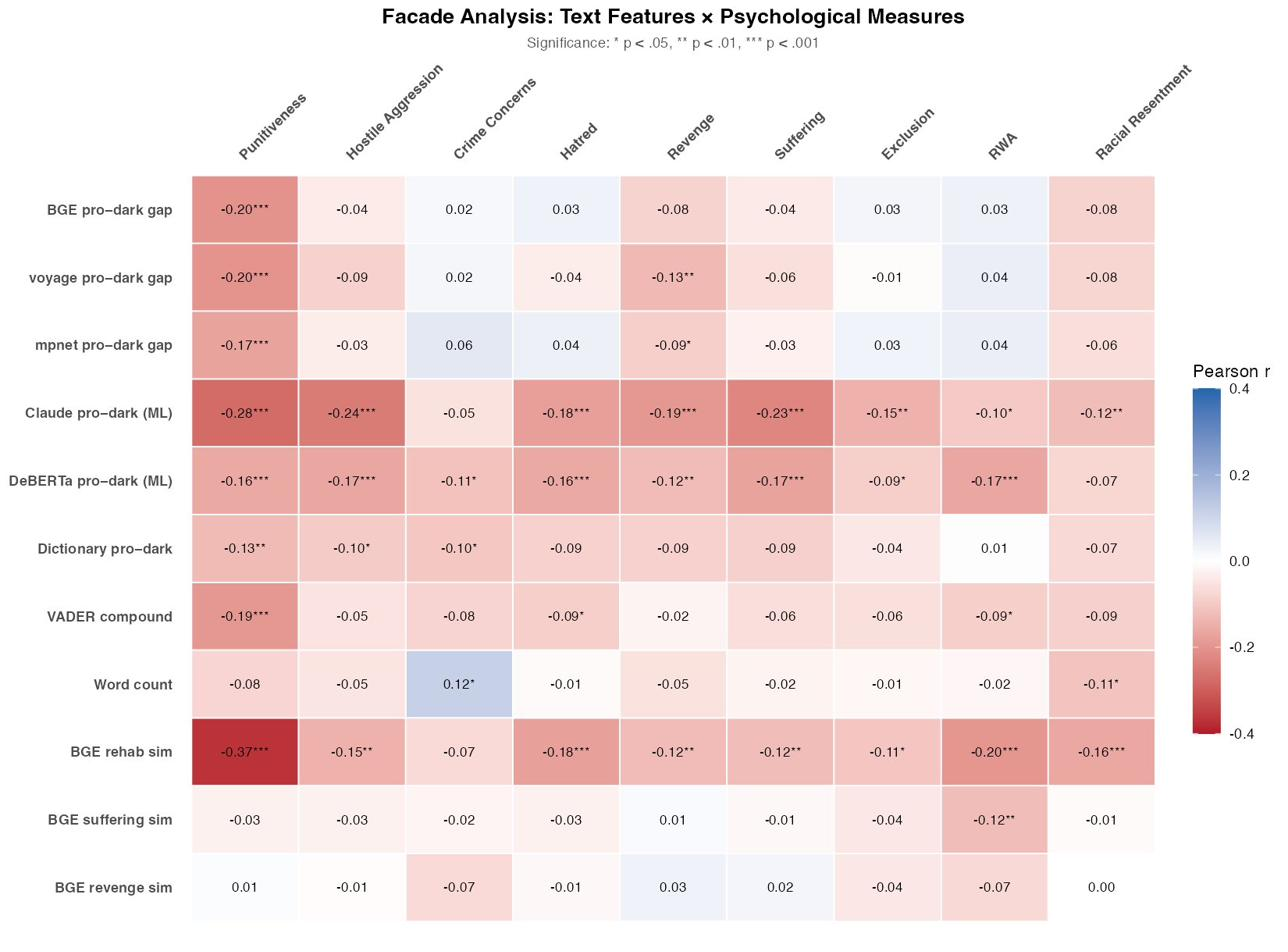
\includegraphics[width=\textwidth]{figures/facade_correlations_heatmap.png}
  \caption{Facade analysis. Pearson correlations between 11 NLP-derived text features (rows) and 9 Study~1 psychological measures (columns). Cell values are correlation coefficients; significance is indicated by stars ($\ast~p < .05$, $\ast\ast~p < .01$, $\ast\ast\ast~p < .001$). Of the 33 cells reaching both statistical significance and a meaningful magnitude threshold ($|r| \geq .10$), 32 are negative. The strongest single cell is BGE rehabilitation similarity $\times$ punitiveness ($r = -.37$). The pattern is incompatible with a simple ``surface tracks substrate'' account: high-punitive and high-hostile participants produce \textit{less} prosocial-sounding language, but they also do not produce more dark-themed language. They selectively suppress rehabilitation-themed language while leaving the other prosocial themes and the dark themes essentially untouched. $N = 496$.}
  \label{fig:facade_heatmap}
\end{figure}
